\documentclass{amsart}
\usepackage[parfill]{parskip} 
\usepackage{amsmath,amssymb,amsthm}
\usepackage[pdftex]{hyperref}
\usepackage{euscript}
\usepackage{tikz-cd}
\usepackage{appendix}
\usepackage{comment}
\usepackage{mathtools}


\hypersetup{
  colorlinks,
  citecolor=blue,
  filecolor=black,
  linkcolor=blue,
  urlcolor=black
}

\theoremstyle{plain}
\newtheorem{theorem}{Theorem}[section]
\newtheorem{corollary}[theorem]{Corollary}
\newtheorem{lemma}[theorem]{Lemma}
\newtheorem{claim}{Claim}


\theoremstyle{definition}
\newtheorem{definition}[theorem]{Definition}

\theoremstyle{remark}
\newtheorem{remark}[theorem]{Remark}
\newtheorem{example}[theorem]{Example}



\def\phi{\varphi}
\def\epsilon{\varepsilon}
\def\E{\exists}
\def\A{\forall}
\DeclareMathOperator{\Clo}{Clo}
\DeclareMathOperator{\Con}{Con}
\DeclareMathOperator{\CSP}{CSP}
\DeclareMathOperator{\Inv}{Inv}
\DeclareMathOperator{\Pol}{Pol}
\DeclareMathOperator{\NP}{NP}
\DeclareMathOperator{\id}{id}
\DeclareMathOperator{\typ}{typ}
\DeclareMathOperator{\End}{End}
\DeclareMathOperator{\Sym}{Sym}
\DeclareMathOperator{\Alg}{Alg}
\DeclareMathOperator{\Eq}{Eq}
\DeclareMathOperator{\Id}{E}
\DeclareMathOperator{\U}{U}
\DeclareMathOperator{\M}{M}
\DeclareMathOperator{\fin}{fin}
\DeclareMathOperator{\SD}{SD}
\DeclareMathOperator{\Sn}{Sn}

\begin{document}
\title{Minimal Algebras}
\author{Arturo}


%\begin{abstract}
  
%\end{abstract}

\maketitle 

\section{Preliminaries} 
\begin{definition}
    Let $F$ be a set of function symbols and $\mathbf{A}$ be an algebra over $F$. 
    We denote by $\Clo(\mathbf{A})$ the smallest set containing 
    \begin{equation*}
        \{f^\mathbf{A}: f \in F\} \quad \text{ and } \quad \{\pi^n_i: A^n \to A, 1 \le i \le n, n \in \omega\}
    \end{equation*}
and closed under composition. 
The elements of $\Clo(\mathbf{A})$ are called \textbf{term} operations. 
We say that two algebras $\mathbf{A}$ and $\mathbf{B}$ on the same carrier are \textbf{term equivalent} if $\Clo(\mathbf{A}) \simeq \Clo(\mathbf{B})$. 
\end{definition}

\begin{definition}
    Let $F$ be a set of function symbols and $\mathbf{A}$ be an algebra over $F$. 
    We denote by $\Pol(\mathbf{A})$ the smallest set containing 
    \begin{enumerate}
        \item $\{f^\mathbf{A}: f \in F\}$; 
        \item $\{\pi^n_i: A^n \to A, 1 \le i \le n, n \in \omega\}$; 
        \item the constant $0$-ary operations
    \end{enumerate}
and closed under composition. 
The elements of $\Pol(\mathbf{A})$ are called \textbf{polynomial} operations. 
We say that two algebras $\mathbf{A}$ and $\mathbf{B}$ on the same carrier are \textbf{polynomially equivalent} if $\Pol(\mathbf{A}) \simeq \Pol(\mathbf{B})$. 
\end{definition}

\begin{example}
    If $\phi \in \Clo_{m+n}(\mathbf{A})$ and $(a_1, \ldots, a_m) \in A^m$, then 
    \begin{equation*}
        \psi: A^n \to A \quad (b_1, \ldots, b_n) \mapsto \phi(a_1, \ldots, a_m,b_1, \ldots, b_n)
    \end{equation*}
is a polynomial operation.  
\end{example}

\begin{remark}
    Let $\mathbf{A}$ be an algebra. 
    An equivalence relation $\alpha$ is a congruence of $\mathbf{A}$ iff $\phi(\alpha) \subseteq \alpha$ for every $\phi \in \Pol_1(\mathbf{A})$. 
\end{remark}

Let $\mathbf{A}$ be a finite algebra. 
We adopt the following convention, concerning the restriction $(-|U)$ operation, for $U \subseteq A$: 
\begin{itemize}
    \item if $\theta \in \Con(\mathbf{A})$, $\theta | U := \theta \cap U^2$; 
    \item if $\phi: A^n \to A$, $\phi|U$ is the function $U^n \to A$, $(u_1, \ldots, u_n) \mapsto \phi(u_1, \ldots, u_n)$; 
    \item $\Pol(\mathbf{A})|U:=\{\psi|U : \psi \in \Pol(\mathbf{A}) \text{ and } \psi[U^n] \subseteq U \}$; 
    \item $\mathbf{A}||U := (U, \Pol(\mathbf{A})|U)$. 
\end{itemize}

\section{Finite Minimal Algebras}
\begin{definition}
    A nontrivial finite algebra $\mathbf{A}$ is \textbf{minimal} iff every noncostant element of $\Pol_1(\mathbf{A})$ is bijective.
\end{definition}

The goal is to classify, up to polynomial equivalence, all the finite minimal algebras. 

\begin{example}
    The following are examples of minimal algebras. 
    \begin{enumerate}
        \item any algebra with carrier $2$; 
        \item a nontrivial finite vector space $\mathbf{A}$ over a finite field $\mathbf{k}$: every $\pi \in \Pol_1(\mathbf{A})$ is of the form $\pi(v)=av+b$ for some $a \in k$, $b \in A$; 
        \item a group of permutations acting on a finite set. If $\mathbf{G}$ is a group acting on a set $A$ 
        each $g \in G$ induces an operation $\phi_g: A \to A$ given by $\phi_g(a)=g \cdot a$. 
        Let $\Phi_\mathbf{G}:=\{\phi_g: g \in G\}$. 
        A $\mathbf{G}$-set can be seen as an algebra $(A, \Phi_\mathbf{G})$.
    \end{enumerate}
\end{example}

We shall see that, up to polynomial equivalence, there are no other finite minimal algebras. 

\begin{lemma}
    Let $\mathbf{A}$ be a minimal algebra.
    If every element of $\Pol(\mathbf{A})$ is essentially unary, then $\mathbf{A}$ is polynomially equivalent to $(A, \Phi_{\mathbf{G}})$ where $\mathbf{G}$ is a finite group acting on $A$. 
    \begin{proof}
        Since $\mathbf{A}$ is minimal, $\Pol_1(\mathbf{A}) \cap \Sym(A)$ is a subgroup of $\Sym(A)$. 
        Let $\mathbf{G}:=\Pol_1(\mathbf{A}) \cap \Sym(A)$. 
        If $\psi \in \Pol(\mathbf{A})$, either $\psi$ is constant or $\psi$ is essentially unary, hence $(A, \Phi_{\mathbf{G}})$ is polynomially equivalent to $\mathbf{A}$. 
    \end{proof}
\end{lemma}

\begin{theorem}
    [\cite{classification-minimal}]
    Let $\mathbf{A}$ be a minimal algebra with $|A| > 2$.  
    If $\Pol(\mathbf{A})$ contains an operation which is not essentially unary, then $\mathbf{A}$ is polynomially equivalent to a $\mathbf{k}$-vector space for a finite field $\mathbf{k}$. 
\end{theorem}

\begin{theorem}
    \label{classification-two}
    Every algebra $\mathbf{A}$ with carrier $2$ is polynomially equivalent to one of the following: 
    \begin{enumerate}
        \item $\mathbf{E}_0= (2, \varnothing)$;
        \item $\mathbf{E}_1 = (2, \lnot)$; 
        \item $\mathbf{E}_3 = (2, \land, \lor, \lnot)$; 
        \item $\mathbf{E}_4 = (2, \land, \lor)$; 
        \item $\mathbf{E}_5 = (2, \lor)$; 
        \item $\mathbf{E}_6 = (2, \land)$.
    \end{enumerate}
    Each of them is not polynomially equivalent to the other\footnote{A classical theorem by Post states that the set of clones of operations on $2$ is countable infinite. 
    By Theorem \ref{classification-two} among these there are exactly seven distinct clones containing the constant operations.
    However it has been proven that the set of clones on $3$ containing the constant operations is uncountable.}.
\end{theorem}

\begin{remark}
    Up to isomorphism, $\mathbf{E}_5 (\simeq \mathbf{E}_6)$ is the only semilattice with two elements, while $\mathbf{E}_3$ and $\mathbf{E}_4$ are the only Boolean algebra and lattice, respectively, with two elements. 
\end{remark}

\begin{definition}
    \label{defn_type}
    Let $\mathbf{A}$ be a minimal algebra. 
    We say that $\mathbf{A}$ is of 
    \begin{enumerate}
        \item \textbf{type 1} (or \textbf{unary}) if $\mathbf{A}$ is polynomially equivalent to $(A, \Phi_\mathbf{G})$ for some $\mathbf{G} \le \Sym(A)$; 
        \item \textbf{type 2} (or \textbf{affine}) if $\mathbf{A}$ is polynomially equivalent to a vector space over a finite field $\mathbf{k}$; 
        \item \textbf{type 3} (or \textbf{Boolean}) if $\mathbf{A}$ is polynomially equivalent to $\mathbf{E}_3$;
        \item \textbf{type 4} (or \textbf{lattice}) if $\mathbf{A}$ is polynomially equivalent to $\mathbf{E}_4$;
        \item \textbf{type 5} (or \textbf{semilattice}) if $\mathbf{A}$ is polynomially equivalent to $\mathbf{E}_5$. 
    \end{enumerate}
\end{definition}

\section{Minimal Algebras Relative to a Congruence}
\begin{definition}
    Let $\mathbf{A}$ be a finite algebra and let $ \theta \in \Con(\mathbf{A}), \Delta_A \neq \theta$. 
    We say that $\mathbf{A}$ is $\theta$-\textbf{minimal} if for all $\epsilon \in \Pol_1(\mathbf{A})$ either $\epsilon$ is bijective or $\epsilon$ is constant on the $\theta$-equivalence classes. 
\end{definition}

\begin{remark}
    Observe that $\mathbf{A}$ is minimal iff $\mathbf{A}$ is $\nabla_A$-minimal. 
\end{remark}

\begin{definition}
    %Let $(\alpha, \beta)$ be tame in a finite algebra $\mathbf{A}$. 
    Let $\mathbf{A}$ be a $\theta$-minimal algebra. 
    A $\theta$-\textbf{trace} of $\mathbf{A}$ is 
    %$N \subseteq A$ such that for some $U \in \M_{\mathbf{A}}(\alpha, \beta)$ and $x \in U$, $N\subseteq U$ and $N=x/(\beta|U) \neq x/(\alpha|U)$. 
    a nontrivial $\theta$-equivalence class.  
    %which contains at least two $\alpha$-equivalence classes. 
\end{definition}

\begin{lemma}
    Let $\mathbf{A}$ be a finite $\theta$-minimal algebra and let $N$ be a $\theta$-trace. 
    Then the algebra $\mathbf{A}||N$ is minimal.
    \begin{proof}
        We need to show that for every 
        \begin{equation*}
            \psi \in \Pol_1(\mathbf{A}||N) = \{ \phi|N : \phi \in \Pol_1(\mathbf{A}), \phi[N] \subseteq N\}
        \end{equation*}
        either $\psi$ is bijective, or $\psi$ is constant. 
        Let $\psi = \phi|N$. 
        Since $\mathbf{A}$ is $\theta$-minimal, either $\phi$ is bijective or $\phi$ is constant on the $\theta$-equivalence classes. 
        Clearly, in the first case $\psi$ is bijective, in the second $\psi$ is constant.  
        %If $\phi(\theta) \subseteq \delta$, $\psi$ is constant: if $(x,y) \in N^2 \subseteq \theta$, then $(\psi(x), \psi(y)) \in \delta$ so that $\psi(x)=\psi(y)$ in $(\mathbf{A}||N)/(\delta|N)$.  
    \end{proof}  
\end{lemma}

\begin{definition}
    Let $\mathbf{A}$ be a finite algebra and $B,C \subseteq A$. 
    We say that $B,C$ are \textbf{polynomially isomorphic} $(B \sim C)$ if there are $\phi, \psi \in \Pol_1(\mathbf{A})$ such that 
    $\phi[B] = C, \psi[C]=B$ and $\psi \phi | B = 1_B, \phi \psi | C = 1_C$. 
\end{definition}

\begin{remark}
    If $B,C \subseteq A$ are polynomial isomorphic in $\mathbf{A}$, then $\mathbf{A}||B \simeq \mathbf{A}||C$. 
    Let $\pi:=\phi|B$, so that $\pi^{-1}=\psi|C$.    
    Of course, $\pi: B \to C$ is a bijection. 
    We show that $\pi$ is a homomorphism. 
    Let $f \in \Pol_n(\mathbf{A})$ such that $f[B^n] \subseteq B$. 
    Then $g(-, \ldots, -):=\pi f(\pi^{-1}(-), \ldots, \pi^{-1}(-)) \in \Pol_n(\mathbf{A})$ too, $g[C^n] \subseteq C$ and 
    \begin{equation*}
        \pi f(b_1, \ldots, b_n) = g(\pi(b_1, \ldots, b_n))
    \end{equation*}
    for all $b_1, \ldots, b_n \in B^n$. 
\end{remark}

\begin{lemma}
    \label{lemma_relative}
    Let $\mathbf{A}$ be a $\theta$-minimal algebra and $N$ be a $\theta$-trace. 
    Then 
    \begin{enumerate}
        \item $(-|N): [\Delta_A, \theta] \to \Con(\mathbf{A}||N)$ is a surjective lattice homomorphism; 
        \item if any two $\theta$-traces are polynomially isomorphic, then it is an isomorphism. 
    \end{enumerate}
    \begin{proof}
        Clearly, the map is well defined and preserves meets. 
        We show that 
        \begin{equation*}
            (\alpha \lor \beta) \cap N^2 = (\alpha \cap N^2) \lor (\beta \cap N^2) \text{.}
        \end{equation*}
        Let $(x,y) \in (\alpha \lor \beta) \cap N^2$. 
        Then there are $x=x_0, \ldots, x_{n+1}=y$ such that either $(x_i,x_{i+1}) \in \alpha$ or $(x_i,x_{i+1}) \in \beta$. 
        We show that for each $i$, $(x_i, x_{i+1}) \in N^2$. 
        Inductively, if $x_i \in N$, and, say, $(x_i, x_{i+1}) \in \alpha \subseteq \theta$, then $x_{i+1} \in N$. 
        Now, for $\beta \in \Con(\mathbf{A}||N)$, let $\hat{\beta}$ be
        \begin{equation*}
            \{(x,y) \in \theta : (\psi(x), \psi(y)) \in N^2 \implies (\psi(x), \psi(y)) \in \beta \quad \A \psi \in \Pol_1(\mathbf{A}) \}
        \end{equation*}
        Then $\hat{\beta}$ is a congruence. 
        We show that $\hat{\beta} \cap N^2 =\beta$, proving surjectivity. 
        If $(x,y) \in \hat{\beta}$, then $(\psi(x), \psi(y)) \in N^2 \implies (\psi(x), \psi(y)) \in \beta$ for all $\psi \in \Pol_1(\mathbf{A})$; 
        if $(x,y) \in N^2$, then $(\psi(x), \psi(y)) \in N^2$. 
        Therefore $(\psi(x), \psi(y)) \in \beta$ for all $\psi \in \Pol_1(\mathbf{A})$, and, taking $\psi(x)=x$, $(x,y) \in \beta$. 
        Conversely, let $(x,y) \in \beta$. As $\beta \subseteq N^2 \subseteq \theta$, $(x,y) \in \theta$. 
        Let $\psi \in \Pol_1(\mathbf{A})$. 
        If $(\psi(x), \psi(y)) \in N^2$, then $\psi \in \Pol_1(\mathbf{A}||N)$. 
        Since $\beta \in \Con(\mathbf{A}||N)$, $ (\psi(x), \psi(y)) \in \beta$.  

        We need to prove injectivity. 
        Let $\alpha < \beta \le \theta$. 
        Let $(x,y) \in \beta - \alpha$. 
        Then $(x,y) \in \theta$ and $P:=x/\theta$ is a $\theta$-trace. 
        Since $P$ is polynomially isomorphic to $N$, there is $\psi \in \Pol_1(\mathbf{A})$ such that 
        \begin{equation*}
            \psi[P] = \psi[x/\theta] =\{\psi(z): (x,z) \in \theta\}= N \text{.}
        \end{equation*}
        Then, $(\psi(x),\psi(y)) \in \theta \cap N^2$.
        Also, $(\psi(x),\psi(y)) \in \beta - \alpha$, so that $(\psi(x),\psi(y)) \in \beta|N - \alpha|N$ and $\alpha|N/< \beta|N$. 
    \end{proof}
\end{lemma}

\begin{lemma}
    Let $\mathbf{A}$ be a $\theta$-minimal algebra with $\Delta_A \prec \theta$. 
    Let $N,K$ be two $\theta$-traces. 
    Then $N$ and $K$ are polynomially isomorphic. 
    \begin{proof}
        Since $\Delta_A \prec \theta$, $\theta_{\mathbf{A}}(N)=\theta$. 
        But $\theta_{\mathbf{A}}(N)$ is the transitive closure of the relation 
        $\{(\psi(x), \psi(y)) : (x,y) \in N^2, \psi \in \Pol_1(\mathbf{A})\}$. 
        Then, as $K$ is a $\theta$-class, there is $\phi \in \Pol_1(\mathbf{A})$ such that $\phi[N] \cap K \neq \varnothing$ 
        and $\phi$ is not constant on $N$. 
        This implies that $\phi \in \Sym(A)$, so that $\phi[N]=K$. 
        Similarly, there is $\psi \in \Pol_1(\mathbf{A}) \cap \Sym(A)$ such that $\psi[N]=K$. 
        Now, $\psi \phi \in \Sym(A)$, hence $(\psi \phi)^k = 1_A$ for some $k > 0$. 
        The polynomials $\phi(\psi \phi)^{k-1}$ and $\psi$ witness that $N \sim K$.
    \end{proof}
\end{lemma}

\section{Minimal Algebras Relative to a Pair} 
\begin{definition}
    Let $\mathbf{A}$ be a finite algebra and let $\delta < \theta \in \Con(\mathbf{A})$. 
    We say that $\mathbf{A}$ is $(\delta, \theta)$-\textbf{minimal} if for all $\epsilon \in \Pol_1(\mathbf{A})$ either $\epsilon$ is bijective or $\epsilon(\theta) \subseteq \delta$. 
\end{definition}

\begin{remark}
    Observe that $\mathbf{A}$ is minimal iff $\mathbf{A}$ is $(\Delta, \nabla)$-minimal. 
\end{remark}

\begin{definition}
    %Let $(\alpha, \beta)$ be tame in a finite algebra $\mathbf{A}$. 
    Let $\mathbf{A}$ be a $(\delta, \theta)$-minimal algebra. 
    An $(\alpha, \beta)$-\textbf{trace} of $\mathbf{A}$ is 
    %$N \subseteq A$ such that for some $U \in \M_{\mathbf{A}}(\alpha, \beta)$ and $x \in U$, $N\subseteq U$ and $N=x/(\beta|U) \neq x/(\alpha|U)$. 
    a $\beta$-equivalence class which contains at least two $\alpha$-equivalence classes. 
\end{definition}

\begin{lemma}
    Let $\mathbf{A}$ be a finite $(\delta,\theta)$-minimal algebra and let $N$ be a $(\delta, \theta)$-trace. 
    Then the algebra $(\mathbf{A}||N)/(\delta|N)$ is minimal.
    \begin{proof}
        We need to show that for every 
        \begin{equation*}
            \psi \in \Pol_1((\mathbf{A}||N)/(\delta|N)) = \{ (\phi|N)/(\delta|N) : \phi \in \Pol_1(\mathbf{A}), \phi[N] \subseteq N\}
        \end{equation*}
        either $\psi$ is bijective, or $\psi$ is constant. 
        Let $\psi = (\phi|N)/(\delta|N)$. 
        Since $\mathbf{A}$ is $(\delta, \theta)$-minimal, either $\phi$ is bijective or $\phi(\theta) \subseteq \delta$. 
        Clearly, if $\phi$ is bijective, $\psi$ is bijective. 
        If $\phi(\theta) \subseteq \delta$, $\psi$ is constant: if $(x,y) \in N^2 \subseteq \theta$, then $(\psi(x), \psi(y)) \in \delta$ so that $\psi(x)=\psi(y)$ in $(\mathbf{A}||N)/(\delta|N)$.  
    \end{proof}  
\end{lemma}

Therefore, with an abuse of language, we shall refer unambiguoulsy to the type of $N$ as the type of $ (\mathbf{A}||N)/(\delta|N)$. 

\begin{theorem}
    Let $\mathbf{A}$ be a $(\delta, \theta)$-minimal algebra. 
    Then all $(\delta, \theta)$-traces of $\mathbf{A}$ have the same type.
\end{theorem}

\begin{definition}
    Let $\mathbf{A}$ be a finite $(\delta, \theta)$-minimal algebra. 
    We say that $\mathbf{A}$ is of type $\mathbf{i}$ relative to $(\delta, \theta)$ if each $(\delta, \theta)$-trace of $\mathbf{A}$ is of type $\mathbf{i}$. 
\end{definition}



\begin{lemma}
    Let $\mathbf{A}$ be a $(\delta, \theta)$-minimal algebra and $N$ be a $(\delta, \theta)$-trace. 
    Then 
    \begin{enumerate}
        \item there is a surjective lattice homomorphism $[\delta, \theta] \to \Con((\mathbf{A}||N)/(\delta|N))$; 
        \item if any two $(\delta, \theta)$-traces are polynomially isomorphic, then it is an isomorphism. 
    \end{enumerate}
    \begin{proof}
        The first part immediately follows from Lemma \ref{lemma_relative}.
        The second is very similar.
        Let $\delta \le \alpha < \beta \le \theta$. 
        Let $(x,y) \in \beta - \alpha$. 
        Then $(x,y) \in \theta - \delta$ and $P:=x/\theta$ is a $(\delta, \theta)$-trace. 
        Since $P$ is polynomially isomorphic to $N$, there is $\psi \in \Pol_1(\mathbf{A})$ such that 
        \begin{equation*}
            \psi[P] = \psi[x/\theta] =\{\psi(z): (x,z) \in \theta\}= N \text{.}
        \end{equation*}
        Then, $(\psi(x),\psi(y)) \in (\theta - \delta) \cap N^2$.
        Also, $(\psi(x),\psi(y)) \in \beta - \alpha$, so that $(\psi(x),\psi(y)) \in \beta|N - \alpha|N$ and $\alpha|N/\delta|N < \beta|N/\delta|N$. 
    \end{proof}
\end{lemma}

The following is an example of a sufficient condition that guarantees that the lattices $[\delta, \theta]$ and $\Con((\mathbf{A}||N)/(\delta|N))$ are isomorphic. 

\begin{lemma}
    Let $\mathbf{A}$ be a $(\delta, \theta)$-minimal algebra with $\delta \prec \theta$. 
    Let $N,K$ be two $(\delta, \theta)$-traces. 
    Then $N$ and $K$ are polynomially isomorphic. 
    \begin{proof}
        Since $\delta \prec \theta$, $\delta \lor \theta_{\mathbf{A}}(N)=\theta$. 
        Then there is $\phi \in \Pol_1(\mathbf{A})$ such that $\phi[N] \cap K \neq \varnothing$ and $\phi[N]^2 \nsubseteq \delta$.
        This implies that $\phi \in \Sym(A)$, so that $\phi[N]=K$ and $N \sim K$.  
    \end{proof}
\end{lemma}

\section{Tame Congruences}

\begin{definition}
    Let $\mathbf{A}$ be a finite algebra and $\alpha, \beta \in \Con(\mathbf{A})$ with $\alpha < \beta$. 
    We denote by
    \begin{enumerate}
        \item $\Id(\mathbf{A})$ the set of $ \epsilon \in \Pol_1(\mathbf{A})$ such that $\epsilon^2 = \epsilon$; 
        \item $\U_{\mathbf{A}}(\alpha, \beta)$ the set $\{\phi[A] : \phi \in \Pol_1(\mathbf{A}), \phi(\beta) \nsubseteq \alpha\}$; 
        \item $\M_{\mathbf{A}}(\alpha, \beta)$ the set of minimal (with respect to the inclusion relation) elements of $\U_{\mathbf{A}}(\alpha, \beta)$. 
    \end{enumerate}
\end{definition}

\begin{remark}
    A finite algebra $\mathbf{A}$ is $(\alpha, \beta)$-minimal iff $A \in \M_{\mathbf{A}}(\alpha, \beta)$. 
    If $\mathbf{A}$ is $(\alpha, \beta)$-minimal, every $\psi \in \M_{\mathbf{A}}(\alpha, \beta)$ such that $\psi(\alpha) \nsubseteq \beta$ is bijective. 
    Clearly $A \in \U_{\mathbf{A}}(\alpha, \beta)$, as witnessed by $\epsilon(x)=x$. 
    If there were $\psi \in \Pol_1(\mathbf{A})$ with $\psi(\alpha) \nsubseteq \beta$ and $\psi[A] \subset A$ we would contradict $(\alpha, \beta)$-minimality. 
    Conversely, let $A \in \M_{\mathbf{A}}(\alpha, \beta)$ and $\psi \in \Pol_1(\mathbf{A})$ with $\psi(\alpha) \nsubseteq \beta$; 
    we show that $\psi \in \Sym(A)$. 
    But by definition of $\M_{\mathbf{A}}(\alpha, \beta)$, there is no $\psi \in \Pol_1(\mathbf{A})$ with $\psi(\alpha) \nsubseteq \beta$ and $\psi[A] \subset A$. 
\end{remark}

%\begin{lemma}
%    Let $\mathbf{A}$ be a finite algebra. 
%    Let $\epsilon \in \Id(\mathbf{A})$, $U=\epsilon[A]$. 
%    Then $(-|U): \Con(\mathbf{A}) \to \Con(\mathbf{A}||U)$ is a surjective lattice homomorphism.
%\end{lemma}

\begin{lemma}
    \label{lemma_ex}
    Let $\epsilon \in \Id(\mathbf{A})$, $U:=\epsilon[A]$, and $\varnothing \neq N \subseteq U$.  
    Then $\mathbf{A}||N = (\mathbf{A}||U)||N$. 
    \begin{proof}
        That $(\Pol(\mathbf{A})|U)|N \subseteq \Pol(\mathbf{A})|N$ is obvious. 
        Conversely, let $\psi=\phi|N$ for some $\phi \in \Pol(\mathbf{A})$ with $\phi[N^k] \subseteq N$. 
        Clearly, $\epsilon \phi [U^k] \subseteq U$. 
        If $(a_1, \ldots, a_k) \in N$, $\phi(a_1, \ldots, a_k) \in N \subseteq U$, hence $\phi(a_1, \ldots, a_k) = \epsilon(a)$ for some $a \in A$. 
        Hence $\epsilon \phi(a_1, \ldots, a_k) = \epsilon^2(a)=\epsilon(a) \in N$ so that $(\epsilon \phi |U )|N = \phi|N$. 
        We have shown that $\psi$ is an operation of $(\mathbf{A}||U)||N$. 
    \end{proof}
\end{lemma}

\begin{definition}
    Let $\mathbf{A}$ be a finite algebra and $\alpha, \beta \in \Con(\mathbf{A})$ with $\alpha < \beta$. 
    The pair $(\alpha, \beta)$ is a pair of \textbf{tame} congruences if there is $V \in \M_{\mathbf{A}}(\alpha, \beta)$, $\epsilon \in \Id(\mathbf{A})$ such that $\epsilon[A]=V$ and 
    $(-|V): [\alpha, \beta] \to [\alpha|V, \beta|V]$ is $0,1$-separating
    
    A lattice homomorphism $\alpha: \mathbf{L} \to \mathbf{N}$ is $0,1$-\textbf{separating} if $\alpha^{-1}[\{\alpha(i)\}]=i$ for $i=0,1$. 
\end{definition}

\begin{theorem}
    Let $(\alpha, \beta)$ be a tame pair of congruences of a finite algebra $\mathbf{A}$.
    For every $U \in \M_{\mathbf{A}}(\alpha, \beta)$, 
    \begin{enumerate} 
        \item there  is $\epsilon \in \Id(\mathbf{A})$ such that $\epsilon[A]=U$; 
        \item $(-|U): [\alpha, \beta] \to \Con(\mathbf{A}||U)$ is a surjective lattice homomorphism which is $0,1$-separating;
        \item $\mathbf{A}||U$ is $(\alpha|U, \beta|U)$-minimal. 
        \item Moreover, any two $(\alpha, \beta)$-minimal sets are polynomially isomorphic. 
    \end{enumerate}
    \begin{proof}
        $(1)$ Since $(\alpha, \beta)$ is tame, there is $V_0 \in \M_\mathbf{A}(\alpha,\beta)$ and $\epsilon_0 \in \Id(\mathbf{A})$ such that $V_0 = \epsilon_0[A]$ and $(-|V_0)$ is $0,1$-separating. 
        \begin{claim}
            \label{lemma_pol_claim1}
            If $(x,y) \in \beta - \alpha$, there is $\phi \in \Pol_1(\mathbf{A})$ with $\phi[A]=V_0$ and such that $(\phi(x), \phi(y)) \in \beta|V_0 - \alpha|V_0$. 
            \begin{proof}
                Let $\theta:=\{(x,y) \in \beta : (\epsilon_0 \phi (x), \epsilon_0 \phi(y)) \in \alpha \text{ for all } \phi \in \Pol_1(\mathbf{A})\}$. 
                Now, $\theta \in [\alpha, \beta]$ and $\alpha |V_0 = \theta|V_0$; 
                that $\alpha |V_0 \subseteq \theta|V_0$ is obvious, for the converse: 
                \begin{align*}
                    \theta|V_0 & = \{ (a,b) \in \beta \cap V^2_0: (\epsilon_0 \phi (a), \epsilon_0 \phi(b)) \in \alpha \quad \A \phi \in \Pol_1(\mathbf{A})\}  \\
                    & = \{(\epsilon_0(x), \epsilon_0(y)) \in \beta : (\epsilon_0 \phi \epsilon_0 (x), \epsilon_0 \phi \epsilon_0 (y)) \in \alpha \quad \A\phi \in \Pol_1(\mathbf{A})\}\\ 
                    & \subseteq \{(\epsilon_0(x), \epsilon_0(y)) \in \beta : (\epsilon_0 (x), \epsilon_0 (y)) \in \alpha \}\\ 
                    & = \{(a,b) \in \beta : (a, b ) \in \alpha \cap V^2_0\}\\ 
                    & = \alpha | V_0 
                \end{align*} 
            This implies that $\theta = \alpha $, since $(-|V_0)$ is $0$-separating. 
            Thus $(x,y) \in \beta - \alpha$ implies $(x,y) \in \beta - \theta$. 
            By definition of $\theta$, there is $\psi \in \Pol_1(\mathbf{A})$ such that $(\epsilon_0 \psi (x), \epsilon_0\psi (y)) \notin \alpha$. 
            Thus $\phi:=\epsilon_0 \psi$ satisfies the conditions $\phi[A] \subseteq V_0$ and $(\phi(x), \phi(y)) \in \beta |V_0 - \alpha|V_0$. 
            Hence $\phi[A] = V_0$ by $(\alpha, \beta)$-minimality. 
            \end{proof}
        \end{claim}
        \begin{claim}
            \label{lemma_pol_claim2}
            The relation $\beta$ is the transitive closure of 
            \begin{equation*}
                \alpha \cup \{(\psi(x), \psi(y)) : (x,y) \in \beta|V_0, \psi \in \Pol_1(\mathbf{A})\} \text{.}
            \end{equation*}
            \begin{proof}
                The transitive closure of $\alpha \cup \{(\psi(x), \psi(y)) : (x,y) \in \beta|V_0, \psi \in \Pol_1(\mathbf{A})\}$ is $\alpha \lor \theta_\mathbf{A}(\beta|V_0)$. 
                But $\alpha \lor \theta_\mathbf{A}(\beta|V_0) \in [\alpha, \beta]$, and therefore, since $(-|V_0)$ is $1$-separating, $\beta=\alpha \lor \theta_\mathbf{A}(\beta|V_0)$. 
            \end{proof}
        \end{claim}
        Assume that $U \in \M_{\mathbf{A}}(\alpha, \beta)$. 
        Then, by definition, there is $\mu \in \Pol_1(\mathbf{A})$ such that $\mu[A] =U$ and $\mu(\beta) \nsubseteq \alpha$. 
        This implies that the equivalence relation 
        \begin{equation*}
            \mu^{-1}(\alpha)=\{(a,b): (\mu(a), \mu(b)) \in \alpha\} 
        \end{equation*}
        is such that $\beta \nsubseteq \mu^{-1}(\alpha)$. 
        Then by Claim \ref{lemma_pol_claim2} there are $a,b \in V_0$ and $\psi \in \Pol_1(\mathbf{A})$ such that $(a,b) \in \beta$ and $(\mu \psi(a), \mu \psi(b)) \notin \alpha$. 
        The function $\mu_1:=\mu \psi \epsilon_0$ satisfies $\mu_1[A] \subseteq U$ and $\mu_1(\beta) \nsubseteq \alpha$: 
        there are $x,y \in A$ such that $(a,b)=(\epsilon_0(x), \epsilon_0(y)) \in \beta $ but $(\mu_1(a), \mu_1(b))=(\mu \psi \epsilon_0(x), \mu \psi \epsilon_0(y)) \notin \alpha$. 
        Thus $\mu_1[A] = U$ by $(\alpha, \beta)$-minimality. 
        Observe that $\mu_1[V_0]=\mu_1 \epsilon_0 [A] = \mu \psi \epsilon^2_0[A] = \mu_1[A]$, so that $\mu_1[V_0] = U$. 
        Apply Claim \ref{lemma_pol_claim1} to the pair $(\mu_1(a), \mu_1(b))$ to get $\nu \in \Pol_1(\mathbf{A})$ such that $\nu[A]=V_0$ and $(\nu \mu_1(a), \nu \mu_1(b)) \notin \alpha$. 
        Now, since $\mu_1 \nu [A] = \mu_1[V_0] = U$, 
        $\mu_1 \nu | U $ is bijective; since $U$ is finite, there is $k >1$ such that $(\mu_1 \nu |U )^k = (\mu_1 \nu)^k |U =1_U$. 
        Let $\epsilon:=(\mu_1 \nu)^k$.
        We have: $\epsilon[A] = (\mu_1 \nu)^k[A]=(\mu_1 \nu)^{k-1}[U]=U$ and, consequently, for all $a \in A$, $\epsilon^2(a)=\epsilon(a)$ since $\epsilon(a) \in U$. 
        Therefore $\epsilon \in \Id(\mathbf{A})$. 

        (2) Clearly, the map is well defined and preserves meets. 
        For $\theta \in [\alpha|U, \beta|U]$, let 
        \begin{equation*}
            \hat{\theta}=\{(x,y) \in \beta : (\epsilon \phi(x), \epsilon \phi(y)) \in \theta \text{ for all } \phi \in \Pol_1(\mathbf{A})\}
        \end{equation*}
        The relation $\hat{\theta}$ is an equivalence relation.
        If $(x,y) \in \hat{\theta}$ and $\psi \in \Pol_1(\mathbf{A})$, then $(\psi(x),\psi(y)) \in \hat{\theta}$ so that $\hat{\theta} \in [\alpha, \beta]$. 
        \textcolor{red}{missing}

        (4) In the above notation, let $\phi:=\nu$, $\psi:=(\mu_1 \nu)^{k-1} \mu_1$. 
        Then $\phi[U] = V_0, \psi[V_0]=U$ and $\psi \phi | U = 1_U, \phi \psi | V_0 = 1_{V_0}$. 
        Then fact that any $(\alpha, \beta)$-minimal set is polynomially isomorphic to $V_0$ implies that any two $(\alpha, \beta)$-minimal sets are polynomially isomorphic. 

        (3) Let $\phi \in \Pol_1(\mathbf{A}||U)=\{\psi|U : \psi \in \Pol_1(\mathbf{A}), \psi[U] \subseteq U\}$. 
        We need to show that if $\phi(\beta | U) \nsubseteq \alpha|U$, then $\phi \in \Sym(U)$. 
        If $\phi(\beta | U) \nsubseteq \alpha|U$, then in particular $\psi(\beta) \nsubseteq \alpha$, so that, by $(\alpha,\beta)$-minimality, $U \subseteq \psi[A]$. 
        Let $\epsilon \in \Id(\mathbf{A})$ such that $\epsilon[A]=U$
        Now, $\phi(\beta | U) \nsubseteq \alpha|U$ is equivalent $\psi \epsilon (\beta) \nsubseteq \alpha$, and $\psi \epsilon[A] \subseteq U$. 
        Then by $(\alpha, \beta)$-minimality, $U =\psi \epsilon[A] = \psi[U]$.  
    \end{proof}
\end{theorem}

\begin{definition}
    Let $(\alpha, \beta)$ be tame in a finite algebra $\mathbf{A}$. 
    An $(\alpha, \beta)$-\textbf{trace$^*$} of $\mathbf{A}$ is 
    $N \subseteq A$ such that for some $U \in \M_{\mathbf{A}}(\alpha, \beta)$ and $x \in U$, $N\subseteq U$ and $N=x/(\beta|U) \neq x/(\alpha|U)$. 
    That is, $N$ is an $(\alpha|U, \beta|U)$-trace of the minimal algebra $\mathbf{A}||U$. 
\end{definition}

\begin{definition}
    Let $(\alpha, \beta)$ be tame in a finite algebra $\mathbf{A}$.
    Let $\delta, \theta \in \Con(\mathbf{A})$. 
    Let $K$ be a class of algebras. 
    We define 
    \begin{enumerate}
        \item the \textbf{type} of $(\alpha, \beta)$, written $\typ(\alpha, \beta)$, to be the type of
        $\mathbf{A}||U$ relative to $(\alpha|U, \beta|U)$;
        \item $\typ\{\delta, \theta\} :=\{ \typ(\alpha, \beta) : \delta \le \alpha \prec \beta \le \beta\}$;
        \item $\typ\{\mathbf{A}\}: =\typ\{\Delta_A, \nabla_A\}$; 
        \item $\typ\{K\}:=\cup\{\typ\{\mathbf{A}\} : \mathbf{A} \in K_{\fin}\}$. 
    \end{enumerate}
    %Let $N$ be a $(\alpha,\beta)$-trace of $\mathbf{A}$. 
    %the minimal algebra $(\mathbf{A}||N)/(\alpha|N)$.
\end{definition}

\begin{remark}
    If $(\Delta, \nabla)$ in $\Con(\mathbf{A})$ is tame, then $\typ(\Delta, \nabla)$ coincides with $\typ(\mathbf{A})$ of Definition \ref{defn_type}. 
\end{remark}

\begin{lemma}
    Let $(\alpha, \beta)$ be tame in a finite algebra $\mathbf{A}$.
    For every $(\alpha, \beta)$-trace$^*$ of $\mathbf{A}$, the algebra $(\mathbf{A}||N)/(\alpha|N)$ is minimal and $\typ(\alpha, \beta) = \typ((\mathbf{A}||N)/(\alpha|N))$. 
    \begin{proof}
        Let $U$ be any $(\alpha, \beta)$-minimal set and $N$ be an $(\alpha|U, \beta|U)$-trace. 
        The algebra $\mathbf{A}||U$ is minimal relative to $(\alpha|U, \beta|U)$. 
        By Lemma \ref{lemma_ex} $\mathbf{A}||N = (\mathbf{A}||U)||N$ and consequently $(\mathbf{A}||N)/(\alpha|N) = ((\mathbf{A}||U)||N)/((\alpha|U)|N)$. 
        The type of $\mathbf{A}||U$ relative to $(\alpha|U, \beta|U)$ is, by definition, the type of the minimal algebra $\mathbf{M}:= ((\mathbf{A}||U)||N)/((\alpha|U)|N)$; 
        but $M$ is the only $(\Delta_M, \nabla_M)$-trace of $\mathbf{M}$, hence this is $\typ(\mathbf{M})$.
    \end{proof}
\end{lemma}

\section{Congruence Lattice Conditions for Omitting Type One}
\begin{definition}
    A lattice $\mathbf{L}$ is \textbf{meet semi-distributive} if it satisfies 
    \begin{equation}
        \label{meet_semi_d}
        a \land b = a \land c \implies a \land b = a \land (b \lor c) 
        \tag{$\SD(\land)$}
    \end{equation}
    for all $a,b,c \in L$. 
    A lattice $\mathbf{L}$ is \textbf{join semi-distributive} if it satisfies $\SD(\lor)$. 
    %We denote by $\mathsf{SD}(\land)$ 
\end{definition}

The smallest lattice satisfying $\SD(\lor)$ but not $\SD(\land)$ is called $\mathbf{D}_1$ and it is depicted in Figure \ref{di_one}.  
\begin{figure}
    \centering
    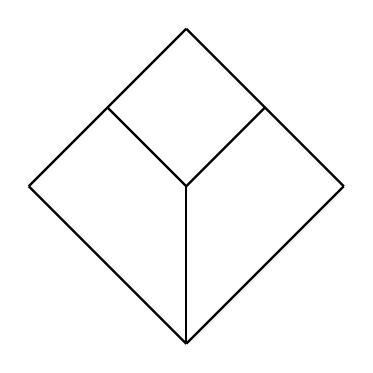
\begin{tikzpicture}
    \label{di_one}
    \draw[black, thick] (0,0) -- (0,-2);
    \draw[black, thick] (0,0) -- (-1,1);
    \draw[black, thick] (0,0) -- (1,1);
    \draw[black, thick] (0,-2) -- (-2,0);
    \draw[black, thick] (0,-2) -- (2,0);
    \draw[black, thick] (-2,0) -- (-1,1);
    \draw[black, thick] (-1,1) -- (0,2);
    \draw[black, thick] (0,2) -- (1,1);
    \draw[black, thick] (1,1) -- (2,0);
    \end{tikzpicture}
    \caption{The lattice $\mathbf{D}_1$.}
\end{figure}

\begin{lemma}
    Let $\mathbf{A}$ be a finite algebra. 
    Suppose that there are $\delta_1, \delta_2, \delta_3 \in \Con(\mathbf{A})$ such that $\Con(\mathbf{A})$ contains an isomorphic copy of $\mathbf{D}_1$, 
    like the fugure below. 
    If $0_{\mathbf{D}_1} \prec \alpha \le \delta_2$, then $\typ(0_{\mathbf{D}_1}, \alpha) = \mathbf{1}$. 
    \begin{figure}
        \centering
        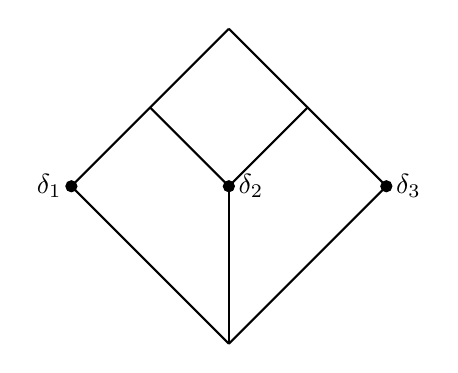
\begin{tikzpicture}
        %\label{di_one}
        \draw[black, thick] (0,0) -- (0,-2);
        \draw[black, thick] (0,0) -- (-1,1);
        \draw[black, thick] (0,0) -- (1,1);
        \draw[black, thick] (0,-2) -- (-2,0);
        \draw[black, thick] (0,-2) -- (2,0);
        \draw[black, thick] (-2,0) -- (-1,1);
        \draw[black, thick] (-1,1) -- (0,2);
        \draw[black, thick] (0,2) -- (1,1);
        \draw[black, thick] (1,1) -- (2,0);
        \filldraw[black] (0,0) circle (2pt) node[anchor=west]{$\delta_2$};
        \filldraw[black] (-2,0) circle (2pt) node[anchor=east]{$\delta_1$};
        \filldraw[black] (2,0) circle (2pt) node[anchor=west]{$\delta_3$};
        \end{tikzpicture}
        %\caption{The lattice $\mathbf{D}_1$.}
    \end{figure}
\end{lemma}

\begin{definition}
    Let $\mathbf{A}$ be a finite algebra. 
    A $1$-\textbf{snag} is a pair $(a,b)$ of distinct elements of $A$ such that for some $\phi \in \Pol_2(\mathbf{A})$ 
    \begin{equation*}
        \phi(a,b)=\phi(b,a)=a \quad \phi(b,b)=b \text{.}
    \end{equation*}
    A $2$-\textbf{snag} is a pair $(a,b)$ of distinct elements of $A$ such that for some $\phi \in \Pol_2(\mathbf{A})$ 
    \begin{equation*}
        \phi(a,b)=\phi(b,a)=\phi(a,a)=a \quad \phi(b,b)=b \text{.}
    \end{equation*}
    We denote by $\Sn_1(\mathbf{A})$ and $\Sn_2(\mathbf{A})$ the set of $1$-snags and $2$-snags, respectively. 
\end{definition}

\begin{remark}
    If $(a,b)$ is a $2$-snag as witnessed by $\phi$, then $\{a,b\}$ is closed under $\phi$ and it is a semilattice. 
\end{remark}

\begin{definition}
    Let $\mathbf{A}$ be a finite algebra. 
    For $\gamma, \delta \in \Con(\mathbf{A})$ we let 
    \begin{align*}
        \gamma \approx \delta & \iff \gamma \cap \Sn_1(\mathbf{A}) = \delta \cap \Sn_1(\mathbf{A})\\
        \gamma \sim \delta & \iff \gamma \cap \Sn_2(\mathbf{A}) = \delta \cap \Sn_2(\mathbf{A})\\
    \end{align*}
\end{definition}

\begin{theorem}
    \label{lemma_msd}
    Let $\mathbf{A}$ be a finite algebra. 
    The relations $\sim$ and $\approx$ are congruences of $\mathbf{L}:=\Con(\mathbf{A})$. 
    The quotient lattice $\mathbf{L}/\sim$ is meet semi-distributive. 
\end{theorem}

\begin{definition}
    Let $K$ be a class of algebras.
    We define $\Con(K):=\{\Con(\mathbf{A}) : \mathbf{A} \in K\}$. 
\end{definition}

\begin{theorem}
    \label{theorem_msd}
    Let $\mathsf{V}$ be a locally finite variety.
    The following are equivalent: 
    \begin{enumerate}
        \item $\mathbf{1} \notin \typ\{\mathsf{V}\}$; 
        \item $\mathbf{D}_1 \notin IS(\Con(\mathsf{V}))$;
        \item for every $\mathbf{A} \in \mathsf{V}$ there is a congruence $\theta$ of $\mathbf{L}:=\Con(\mathbf{A})$ such that 
        $\mathbf{L}/\theta$ is meet semi-distributive and for all $a \in L$, $a / \theta$ is modular; 
        \item for every $\mathbf{A} \in \mathsf{V}$, if $\alpha, \beta \in \Con(\mathbf{A})$ are such that $\alpha \sim \beta$, then $\alpha \circ \beta = \beta \circ \alpha$; 
        \item there is an idempotent term $t$ such that for every $\mathbf{A} \in \mathsf{V}$, if $\Delta_A \sim \theta \in \Con(\mathbf{A})$, then
        \begin{equation*}
            t^\mathbf{A}(a,b,b)=a \quad t^{\mathbf{A}}(a,a,b)=b 
        \end{equation*}
        for all $(a,b) \in \theta$, i.e. $t$ is a Mal'cev term on the $\theta$-equivalence classes. 
    \end{enumerate}
\end{theorem}


\section{Syntactic Conditions for Omitting Type One}

\begin{definition}
    Let $\mathsf{V}$ be a variety. 
    An algebra $\mathbf{A} \in \mathsf{V}$ is called
    \begin{enumerate}
        \item \textbf{free} if there is an isomorphism $\mathbf{A} \simeq \mathbf{F}_{\mathsf{V}}(\kappa)$ for some cardinal $\kappa$; 
        \item \textbf{finitely generated} if there is a surjective homomorphism $\mathbf{F}_{\mathsf{V}}(n) \to \mathbf{A}$ for some $n \in \omega$. 
    \end{enumerate} 
\end{definition}

\begin{definition}
    A variety $\mathsf{V}$ is called 
    \begin{enumerate}
    \item \textbf{locally finite} if all its finitely generated algebras are finite; 
    \item \textbf{finitely presented} if $\mathsf{V}$ has a finite set of function symbols and $\mathsf{V}= \Alg(\Sigma)$ for a finite set of equations $\Sigma$; 
    \item \textbf{finitely generated} if $\mathsf{V}=V(\mathbf{A}_1, \ldots, \mathbf{A}_n)$ for $\mathbf{A}_1, \ldots, \mathbf{A}_n$ finite similar algebras; 
    \item \textbf{linear} if there is a set of equations defining $\mathsf{V}$ containing at most one function symbol per side. 
    \end{enumerate}
\end{definition}

\begin{remark}
    Observe that $V(\mathbf{A}_1, \ldots, \mathbf{A}_n)=V(\mathbf{A}_1 \times \cdots \times \mathbf{A}_n)$.  
\end{remark}

\begin{lemma}
    \label{loc_fin}
    Let $\mathsf{V}$ be a variety. 
    If $\mathsf{V}$ is finitely generated then it is locally finite. 
    \begin{proof}
        %Let $\mathsf{V}=HSP(\mathbf{A}_1, \ldots, \mathbf{A}_n)$ with $\mathbf{A}_i$ finite. 
        %Let $\mathbf{A} \in \mathsf{V}$ be finitely generated. 
        %Then there is a surjective homomorphism $\alpha: \mathbf{A}' \to \mathbf{A}$ for some 
        %\begin{equation*}
        %    \mathbf{A}' \le \mathbf{A}^{\kappa_1}_1 \times \cdots \times \mathbf{A}^{\kappa_n}_n
        %\end{equation*} 
        %We prove that $\mathbf{A}'$ is finite. 
        %Without loss of generality we can assume that $\mathbf{A}'$ is finitely generated: if not we can replace $\mathbf{A}'$ with $\mathbf{A}' /\ker(\alpha)$. 
        %Since $\mathbf{A}'$ is finitely generated, 
        %there is a finite number of homomorphisms $\mathbf{A}' \to \mathbf{A}_i$ for every $i$. 
        %Composing the embedding 
        %\begin{equation*}
        %    \mathbf{A}' \hookrightarrow  \mathbf{A}^{\kappa_1}_1 \times \cdots \times \mathbf{A}^{\kappa_n}_n
        %\end{equation*} with the projections, 
        %we see that $\mathbf{A}'$ embeds into $\mathbf{A}^{k_1}_1 \times \cdots \times \mathbf{A}^{k_n}_n$ for some \emph{finite} $k_1, \ldots, k_n$, hence it is finite. 
    
        By the previuos remark, we can assume that $\mathsf{V}=V(\mathbf{A})$ for some $\mathbf{A}$ finite. 
        Let $n < \omega$. 
        We prove that $\mathbf{F}_{\mathsf{V}}(n)$ is finite. 
        Consider the homomorphism
        \begin{equation*}
            \mathbf{F}_{\mathsf{V}}(n) \to \mathbf{A}^{A^n}, \quad t(x_1, \ldots, x_n) \mapsto t^\mathbf{A}
        \end{equation*}
        This homomorphism is injective: if $t^\mathbf{A} = s^\mathbf{A}$, then $\mathbf{A} \models t \equiv s$, i.e. $t=s$ in $\mathbf{F}_{\mathsf{V}}(n)$. 
        %between $\mathbf{F}_{\mathsf{V}}(n)$ and the subalgebra of $\mathbf{A}^{A^n}$ with underlying set $\Clo_n(\mathbf{A})$. 
        Thus $\mathbf{F}_{\mathsf{V}}(n)$ is finite. 
    \end{proof}
\end{lemma}

\begin{definition}
    Let $\mathsf{V}$ and $\mathsf{W}$ be two varieties. 
    We say that $\mathsf{V}$ is \textbf{interpretable} into $\mathsf{W}$ ($\mathsf{V} \le \mathsf{W}$) if there is a clone homomorphism $\Clo(\mathsf{V}) \to \Clo(\mathsf{W})$. 
\end{definition}

\begin{remark}
    Let $\mathsf{W}, \mathsf{V}$ be two varieties. 
    We unravel what $\mathsf{V} \le \mathsf{W}$ means in a simple case, that is when $\mathsf{V}$ is finitely presented. 
    Let $F$ be a finite set of function symbols.
    Let $\mathsf{V}$ be a variety of algebras over $F$, defined by the equations 
    \begin{equation}
        \label{remark_clone}
        s_1 \equiv t_1,\ldots, s_k \equiv t_k \tag{$\star$}\text{.}
    \end{equation} 
    Assume that for each $f \in F_n$ there is $t \in \Clo_n(\mathsf{W})$ such that the interpetation of the $t$'s satisfy the equations \eqref{remark_clone}. 
    Then the assignment $f \mapsto t$ extends to a clone homomorphism $\Clo(\mathsf{V}) \to \Clo(\mathsf{W})$. 
    Of course, the converse also holds; thus this is equivalent to $\mathsf{V} \le \mathsf{W}$. 
\end{remark}

\begin{lemma}
    \label{trivial_pol}
    Let $\mathbf{M}$ be finite minimal algebra of type $\mathbf{1}$. 
    Let $\mathbf{A}=(M, \Pol(\mathbf{M}))$.
    Then $V(\mathbf{A})$ contains a finite algebra $\mathbf{S}$ all of whose polynomials are constant or projections. 
    \begin{proof}
        Let $\mathbf{G}:=\Sym(M) \cap \Pol_1(\mathbf{M})$, subgroup of $\Sym(M)$. 
        Let $u,v \in M$, $u \neq v$ and let 
        \begin{equation*}
            D:=\{(\sigma(u), \sigma(v)) : \sigma \in \mathbf{G}\} \cup \{(\sigma(v), \sigma(u)) : \sigma \in \mathbf{G}\}
        \end{equation*}
        Since $\mathbf{M}$ is minimal with $\typ(\mathbf{M})=\mathbf{1}$, every polynomial $\psi$ is constant or there is $i$, $\sigma \in \mathbf{G}$ such that 
        \begin{equation*}
            \psi(a_1, \ldots, a_n) = \sigma(a_i) \text{.}
        \end{equation*}
        This implies that $\mathbf{D}$ is a subalgebra of $\mathbf{A}^2$. 
        Let 
        \begin{equation*}
            ((x_1, x_2), (y_1,y_2)) \in \theta \iff \sigma(x_i)=y_i \text{ for some } \sigma \in \mathbf{G}
        \end{equation*}
        We show that every term operation of $\mathbf{D}/\theta$ is either constant or a projection. 
        Let $\psi \in \Pol_n(\mathbf{M})$ non constant and $(a_i,b_i) \in D$ for $i=1, \ldots, n$. 
        Then there is $\tau \in \mathbf{G}$ such that 
        \begin{align*}
           \psi((a_1, b_1)/\theta, \ldots, (a_n, b_n)/\theta) & = \psi((a_1, b_1), \ldots, (a_n, b_n)) /\theta \\
           & = (\psi(a_1, \ldots, a_n), \psi(b_1,\ldots, b_n)) / \theta \\
           & = (\tau(a_i), \tau(b_i)) / \theta \\
           & = (a_i, b_i) / \theta \text{.} \qedhere \\
        \end{align*}
    \end{proof}
\end{lemma}

\begin{lemma}
    \label{lemma_type1}
    Let $\mathsf{W}, \mathsf{V}$ be two varieties such that $\mathsf{W} \le \mathsf{V}$. 
    Assume that $\mathsf{W}$ is 
    \begin{itemize}
        \item idempotent; 
        \item finitely presented; 
        \item linear. 
    \end{itemize}
    Let $\mathbf{A} \in \mathsf{V}$, $\epsilon \in \Id(\mathbf{A})$, $U:=\epsilon[A]$, $\beta \in \Con(\mathbf{A})$ and $N:=a/\beta \cap U$ for $a \in U$. 
    Then $\mathsf{W} \le V(\mathbf{A}||N)$. 
    Moreover, if $\mathbf{1} \in \typ\{\mathsf{V}\}$, then $\mathsf{W} \le \mathsf{Set}$. 
    \begin{proof}
        By assumption $\mathsf{W}$ can be described by a finite set of equations of the form 
        \begin{equation}
            f_i(x_{i_1}, \ldots, x_{i_h}) \equiv f_j(x_{j_1}, \ldots, x_{j_k})
        \end{equation}
        where $f_i$ and $f_j$ are members of a finite set $F$ of function symbols. 
        Since $\mathsf{W} \le  \mathsf{V}$, there is an assignment $f \mapsto t$ extending to a clone homomorphism. 
        We need to find a clone homomorphism $\Clo(\mathsf{W}) \to \Clo(\mathbf{A}||N)$. 
        Consider $f \mapsto \phi:=\epsilon t^\mathbf{A} |N$. 
        Firstly, it is well defined: if $(a_1, \ldots, a_n) \in N$, $(\phi(a_1, \ldots, a_n), \phi(a, \ldots, a)) \in \beta$ but 
        \begin{equation*}
            \phi(a, \ldots, a) = \epsilon t^\mathbf{A} (a, \ldots, a) = \epsilon(a)=a \in U
        \end{equation*}
        so that $\phi(a_1, \ldots, a_n) \in N$ and therefore $\phi \in \Pol(\mathbf{A})|N$. 
        Finally, using that $\mathsf{W} \le  \mathsf{V}$, for every $a_{i_1}, \ldots, a_{i_h},a_{j_1}, \ldots, a_{j_k} \in N$
        \begin{align*}
            \phi_i(a_{i_1}, \ldots, a_{i_h}) & = \epsilon t_i^\mathbf{A} (a_{i_1}, \ldots, a_{i_h}) \\
            & = \epsilon t_j^\mathbf{A} (a_{j_1}, \ldots, a_{j_k})\\
            & = \phi_j(a_{j_1}, \ldots, a_{j_k}) \text{.} \\
        \end{align*} 
        If $\mathbf{1} \in \typ\{\mathsf{V}\}$, 
        then there is $\mathbf{A} \in \mathsf{V}$ and $\alpha \prec \beta \in \Con(\mathbf{A})$ such that $\typ(\alpha, \beta) =\mathbf{1}$. 
        Without loss of generality we can assume that $\alpha = \Delta_A$. 
        Let $N$ be a $(\Delta_A, \beta)$-trace$^{*}$.
        Then there are $\epsilon \in \Id(\mathbf{A})$, $U:=\epsilon[A]$ such that $N = a /\beta \cap U$ for some $a \in U$. 
        Thus $\mathsf{W} \le V(\mathbf{A}||N)$. 
        The algebra $\mathbf{A}||N$ is minimal of type $\typ(\Delta_A,\beta)=\mathbf{1}$. 
        Hence by Lemma \ref{trivial_pol}
        there is $\mathbf{S} \in V(\mathbf{A}||N)$ such that every term operation of $\mathbf{S}$ is constant or a projection. 
        Then there is a clone homomorphism $\Clo(\mathbf{A}||N) \to \Clo(\mathbf{S})$.
        Since $\mathsf{W} \le V(\mathbf{A}||N)$ there is a clone homomorphism $\Clo(\mathsf{W}) \to \Clo(\mathbf{A}||N)$. 
        Thus we get a clone homomorphism $\Clo(\mathsf{W}) \to \Clo(\mathbf{S})$. 
        But for every $f \in F$, $\mathsf{W}$ satisfies $f(x, \ldots, x) \equiv x$, hence the image of $f$ through this clone homomorphism cannot be but a projection. 
        This implies that $\mathsf{W} \le \mathsf{Set}$. 
    \end{proof}
\end{lemma}

\begin{lemma}
    \label{lemma_linear}
    Let $\mathsf{V}$ be an idempotent variety over the set of function symbols $F$. 
    Then the following are equivalent: 
    \begin{enumerate}
        \item $\mathsf{V} \nleq \mathsf{Set}$; 
        \item there is an idempotent, finitely presented, linear vareity $\mathsf{W}$ such that $\mathsf{W} \le \mathsf{V}$ but $\mathsf{W} \nleq \mathsf{Set}$; 
        \item $F$ is nonempty and $\mathsf{V}$ satisfies the equations 
        \begin{align}
            \label{linear_eq}
            f(x_{11}, \ldots, x_{1n}) & \equiv f(y_{11}, \ldots, y_{1n}) \notag\\
            & \vdotswithin{\equiv} \tag{$\triangle$}  \\ 
            f(x_{n1}, \ldots, x_{nn}) & \equiv f(y_{n1}, \ldots, y_{nn}) \notag
        \end{align}
        for some $n >0$ and $x_{ii} \neq y_{ii}$. 
    \end{enumerate}
    \begin{proof}
        Firstly, we prove that $(3)$ implies $(2)$. 
        Let $\mathsf{W}$ be the variety over $\{f\}$ defined by the equations \eqref{linear_eq}. 
        Then $\mathsf{W}$ is idempotent, finitely presented and linear. 
        Clearly, $\mathsf{W} \le \mathsf{V}$ but $\mathsf{W} \nleq \mathsf{Set}$. 

        The implication ``$(2) \implies (1)$" is obvious. 

        If $\mathsf{V} \nleq \mathsf{Set}$
    \end{proof}
\end{lemma}

\begin{theorem}
    \label{omitting_typ1}
    Let $\mathsf{V}$ be a locally finite variety. 
    The following are equivalent: 
    \begin{enumerate}
        \item $\mathbf{1} \notin \typ\{\mathsf{V}\}$; 
        \item there is an idempotent variety $\mathsf{W}$ such that $\mathsf{W} \le \mathsf{V}$ and $\mathsf{W} \nleq \mathsf{Set}$. 
        \item there is $m > 0$ such that for every $\mathbf{A} \in \mathsf{V}$, $\alpha, \beta, \gamma \in \Con(\mathbf{A})$ 
        \begin{equation*}
            \alpha \land (\beta \circ \gamma) \le \gamma_m \circ \beta_m 
        \end{equation*}
        where 
        \begin{equation*}
        \begin{cases}
            (\beta_0, \gamma_0) = (\beta, \gamma) \\
            (\beta_{n+1}, \gamma_{n+1})  = (\beta \lor (\alpha \land \gamma_n), \gamma \lor (\alpha \land \beta_n)) \\
        \end{cases}
    \end{equation*}
    \end{enumerate}
    \begin{proof}
        $(2) \implies (1)$: if there is $\mathsf{W}$ idempontent such that $\mathsf{W} \nleq \mathsf{Set}$, 
        then there is $\mathsf{W}'$ idempotent, finitely presented, linear such that $\mathsf{W}' \le \mathsf{W}$, $\mathsf{W}' \nleq \mathsf{Set}$ by Lemma \ref{lemma_linear}. 
        Assume that $\mathbf{1} \in \typ{\mathsf{V}}$, then by Lemma \ref{lemma_type1}, $\mathsf{W}' \le \mathsf{Set}$.
        Absurd.  

        $(1) \implies (3)$: consider the algebra $\mathbf{F}_{\mathsf{V}}(x,y,z) \in \mathsf{V}$. 
        Let $\alpha:=\theta(x,z), \beta:=\theta(x,y), \gamma:=\theta(y,z)$ and $(\beta_n), (\gamma_n)$ as above. 
        By induction, the two sequences $(\beta_n), (\gamma_n)$ are increasing. 
        Since $\mathbf{F}_{\mathsf{V}}(x,y,z)$ is finite, there is $m > 0$ such that $\beta_m = \beta_{m+1}$, $\gamma_m = \gamma_{m+1}$. 
        Then 
        \begin{align*}
            \alpha \land \gamma_m & \le \beta \lor (\alpha \land \gamma_m) = \beta_m \\
            \alpha \land \beta_m & \le \beta \lor (\alpha \land \beta_m) = \gamma_m
        \end{align*}
        so that $\alpha \land \beta_m = \alpha \land \gamma_m$. 
        By Lemma \ref{lemma_msd}, $\Con(\mathbf{F}_{\mathsf{V}}(x,y,x))/ \sim$ is meet semi-distributive, so that 
        \begin{equation*}
            \alpha \land \beta_m \sim \alpha \land (\beta_m \lor \gamma_m) \text{.}
        \end{equation*}
        \begin{claim}
            $\gamma_m \sim \beta_m$ 
        \end{claim}
        By Theorem \ref{theorem_msd}, this implies that $\gamma_m \circ \beta_m = \beta_m \circ \gamma_m$. 
        Since $(x,z) \in \beta \circ \gamma \le \beta_m \circ \gamma_m$, $(x,z) \in \gamma_m \circ \beta_m$.
        Now, let $\mathbf{A} \in \mathsf{V}$. 
        Let $\alpha, \beta, \gamma \in \Con(\mathbf{A})$ and $(a,c) \in \alpha \land (\beta \circ \gamma)$. 
        Let $b \in A$ such that $(a,b) \in \beta, (b,c) \in \gamma$. 
        Let $f: \mathbf{F}_{\mathsf{V}}(x,y,z) \to \mathbf{A}$ be the homomorphism
        \begin{equation*}
            x \mapsto a, y \mapsto b, z \mapsto c \text{.}
        \end{equation*} 
        Now, the function $\theta \mapsto f^{-1}(\theta)$ is an isomorphism of lattices 
        \begin{equation*}
            \Con(\mathbf{A}) \simeq [f^{-1}(\Delta_A), \nabla_A] \text{.}
        \end{equation*}
        Consequently, as $\theta(x,z) \subseteq f^{-1}(\alpha)$, $\theta(x,y) \subseteq f^{-1}(\beta)$, $\theta(y,z) \subseteq f^{-1}(\gamma)$, by induction  
        $\theta(x,z)_m \subseteq f^{-1}(\alpha_m)$, $\theta(x,y)_m \subseteq f^{-1}(\beta_m)$, $\theta(y,z)_m \subseteq f^{-1}(\gamma_m)$.
        Then $f(\theta(y,z)_m \circ \theta(x,y)_m) \subseteq \gamma_m \circ \beta_m$ and therefore $(a,c) \in \gamma_m \circ \beta_m$. 

        $(3) \implies (2)$:
    \end{proof}
\end{theorem}

\begin{corollary}
    Let $\mathbf{A}$ be a finite idempotent algebra. 
    There is $\mathbf{B} \in HS(\mathbf{A})$ such that $\Clo(\mathbf{B}) \simeq \mathbf{N}$ iff $\mathbf{1} \in \typ\{HS(\mathbf{A})\}$. 
    \begin{proof}
        If $\mathbf{1} \in \typ\{HS(\mathbf{A})\}$, then $\mathbf{1} \in \typ\{V(\mathbf{A})\}$. 
        Since $\mathbf{A}$ is finite, then, by Lemma \ref{loc_fin} $V(\mathbf{A})$ is locally finite, 
        and therefore, by Theorem \ref{omitting_typ1}, for every idempotent variety $\mathsf{W}$, either $\mathsf{W} \nleq V(\mathbf{A})$ or $\mathsf{W} \le \mathsf{Set}$. 
        In particular, since $\mathbf{A}$ is idempotent, $V(\mathbf{A}) \le \mathsf{Set}$. 
        This means that there is a clone homomorphism $\Clo(\mathbf{A}) \to \mathbf{N}$. 
        Therefore, there is $\mathbf{S} \in \mathsf{Set}$ such that $\mathbf{S} \in V(\mathbf{A})$. 
        %Without loss of generality, we can assume that $\mathbf{S}$ is finite. 
        \textcolor{red}{missing}

        Conversely, let $\mathbf{B} \in HS(\mathbf{A})$ such that $\Clo(\mathbf{B}) \simeq \mathbf{N}$; 
        this means that $\mathbf{B} \in \mathsf{Set}$ and therefore $\mathbf{B}$ is minimal of type $\mathbf{1}$. 
        %this means that $\mathbf{B}$ is term equivalent to a set. 
        %Hence $\mathbf{B}$ is polynomially equivalent to a set on which the trivial group acts. 
        %Then $\mathbf{1} \in \typ\{\mathbf{B}\}$, and therefore $\mathbf{1} \in \typ\{HS(\mathbf{A})\}$. 
    \end{proof}
\end{corollary}

\begin{definition}
    Let $\mathbf{A}$ be an algebra and $\mathsf{V}$ be a variety. 
    Let $t=t(x_1, \ldots, x_n)$ with $n >0$.
    We say that $t$ is a
    \begin{enumerate}
        \item \textbf{Taylor} term 
        \item \textbf{weak near-unanimity} term 
    \end{enumerate}
    for $\mathbf{A}$ (or $\mathsf{V}$) if $\mathbf{A}$ (or $\mathsf{V}$) satisfies 
    \begin{enumerate}
        \item $t(x_1, \ldots, x_n) \equiv t(y_1, \ldots, y_n)$ with $x_i, y_i \in \{x,y\}$ and $x_i \neq y_i$;
        \item $t(y, x, \ldots, x) \equiv t(x,y,x,\ldots, x) \equiv \cdots \equiv t(x, \ldots, x,y)$
    \end{enumerate}
    respectively. 
\end{definition}

\begin{theorem}
    Let $\mathsf{V}$ be a locally finite variety. The following are equivalent: 
    \begin{enumerate}
        \item $\mathbf{1} \notin \typ\{\mathsf{V}\}$; 
        \item $\mathsf{V}$ has an $n$-ary Taylor idempotent term for some $n >1$. 
    \end{enumerate}
\end{theorem}

\begin{theorem}
    [\cite{wnu}]
    Let $\mathsf{V}$ be a locally finite variety. The following are equivalent: 
    \begin{enumerate}
        \item $\mathbf{1} \notin \typ\{\mathsf{V}\}$; 
        \item $\mathsf{V}$ has an $n$-ary weak near-unanimity idempotent term for some $n >1$. 
    \end{enumerate}
\end{theorem}

\begin{corollary}
    Let $\mathbf{A}$ be a finite idempotent algebra. 
    Then $\Clo(\mathbf{A})$ contains a weak near-unanimity operation iff $\mathbf{1} \notin \typ\{HS(\mathbf{A})\}$. 
\end{corollary}

\begin{theorem}
    [\cite{siggers}]
    Let $\mathsf{V}$ be a locally finite variety.
    The following are equivalent: 
    \begin{enumerate}
        \item $\mathbf{1} \notin \typ\{\mathsf{V}\}$; 
        \item $\mathsf{V}$ has an idempotent $6$-ary term $t$ such that $\mathsf{V}$ satisfies 
    \begin{equation*}
        t(x,x,x,x,y,y) \equiv t(x,y,x,y,x,x) \text{, } t(y,y,x,x,x,x) \equiv t(x,x,y,x,y,x)
    \end{equation*}
    \end{enumerate}
\end{theorem}


\begin{center}
\begin{tikzpicture}
    %\filldraw[black] (0,0) circle (2pt)
    %\filldraw[black] (-1,1) circle (2pt);
    %\filldraw[black] (0,-2) circle (2pt);
    %\filldraw[black] (1,1) circle (2pt);
    %\filldraw[black] (2,0) circle (2pt);
    %\filldraw[black] (0,2) circle (2pt);
    %\filldraw[black] (0,-2) circle (2pt);
\end{tikzpicture}
\end{center} 


\begin{thebibliography}{9}
    \bibitem{finite}
    Hobby, D., McKenzie, R. (1988). \emph{The structure of Finite Algebras}. Contemporary Mathematics 76, American Mathematical Society.  
    \bibitem{wnu}
    Mar\'oti, M., McKenzie, R. (2008). Existence theorems for weakly symmetric operations. \emph{Algebra Universalis} 59, 463-489.
    \bibitem{classification-minimal} 
    P\'alfy, P. P. (1984). Unary polynomials in algebras I. \emph{Algebra Universalis} 18, 262-273.
    %\bibitem{classification}
    %Szendrei, Á. (1990). Simple surjective algebras having no proper subalgebras. \emph{Journal of the Australian Mathematical Society}, 48(3), 434-454. 
    \bibitem{siggers}
    Siggers, M. H. (2010). A strong Mal'cev condition for locally finite varieties omitting the unary type. \emph{Algebra Universalis} 64, 15-20.
 \end{thebibliography}
\end{document}